% !TEX root = /home/fred-olav/afgv/src/preamble.tex
% Start preamble
\documentclass[10pt,a5paper,norsk]{article}
\usepackage{geometry}
 \geometry{
 a5paper,
 total={120mm,185mm},
 left=10mm,
 top=10mm,
 }
\usepackage[utf8]{inputenc}
\usepackage[table]{xcolor}
\usepackage[T1]{fontenc}
\usepackage[pdftex]{graphicx}
\graphicspath{{./}}
\usepackage{enumitem}
\usepackage{pdfpages}
\usepackage{hyperref}
\usepackage{tikz}
\usepackage{attachfile}
\usepackage[ngerman]{babel}
\usepackage{epstopdf}
\usepackage{array}
\usepackage{longtable}
%\usepackage[table,xcdraw]{xcolor}
\usepackage{amsmath}
\usepackage{makecell}
\usepackage{multirow}
%\setlength{\textwidth}{11cm}
%\setlength{\oddsidemargin}{-0.5cm}
\setlength{\evensidemargin}{-1.5cm}
%\setlenght{\headsep}{0cm}
\setlength\parindent{0pt}
%\setlength{\extrarowheight}{3pt}
\usepackage{listings}
\usepackage{microtype}
\usepackage{setspace}
\usepackage{verbatim}
\usepackage{wrapfig}
%\usepackage{xcolor}

 %%%%%%%%%%%%%%%%%%%%%%%%%%%%%%%%%%%%%%%%%%%%%%%%%%%%%%%%%%%%%%%%%%%%%%%%%%%%%%%% 
%%% ~ Arduino Language - Arduino IDE Colors ~                                  %%%
%%%                                                                            %%%
%%% Kyle Rocha-Brownell | 10/2/2017 | No Licence                               %%%
%%% -------------------------------------------------------------------------- %%%
%%%                                                                            %%%
%%% Place this file in your working directory (next to the latex file you're   %%%
%%% working on).  To add it to your project, place:                            %%%
%%%     %%%%%%%%%%%%%%%%%%%%%%%%%%%%%%%%%%%%%%%%%%%%%%%%%%%%%%%%%%%%%%%%%%%%%%%%%%%%%%%% 
%%% ~ Arduino Language - Arduino IDE Colors ~                                  %%%
%%%                                                                            %%%
%%% Kyle Rocha-Brownell | 10/2/2017 | No Licence                               %%%
%%% -------------------------------------------------------------------------- %%%
%%%                                                                            %%%
%%% Place this file in your working directory (next to the latex file you're   %%%
%%% working on).  To add it to your project, place:                            %%%
%%%     %%%%%%%%%%%%%%%%%%%%%%%%%%%%%%%%%%%%%%%%%%%%%%%%%%%%%%%%%%%%%%%%%%%%%%%%%%%%%%%% 
%%% ~ Arduino Language - Arduino IDE Colors ~                                  %%%
%%%                                                                            %%%
%%% Kyle Rocha-Brownell | 10/2/2017 | No Licence                               %%%
%%% -------------------------------------------------------------------------- %%%
%%%                                                                            %%%
%%% Place this file in your working directory (next to the latex file you're   %%%
%%% working on).  To add it to your project, place:                            %%%
%%%    \input{arduinoLanguage.tex}                                             %%%
%%% somewhere before \begin{document} in your latex file.                      %%%
%%%                                                                            %%%
%%% In your document, place your arduino code between:                         %%%
%%%   \begin{lstlisting}[language=Arduino]                                     %%%
%%% and:                                                                       %%%
%%%   \end{lstlisting}                                                         %%%
%%%                                                                            %%%
%%% Or create your own style to add non-built-in functions and variables.      %%%
%%%                                                                            %%%
 %%%%%%%%%%%%%%%%%%%%%%%%%%%%%%%%%%%%%%%%%%%%%%%%%%%%%%%%%%%%%%%%%%%%%%%%%%%%%%%% 

\usepackage{color}
\usepackage{listings}    
\usepackage{courier}

%%% Define Custom IDE Colors %%%
\definecolor{arduinoGreen}    {rgb} {0.17, 0.43, 0.01}
\definecolor{arduinoGrey}     {rgb} {0.47, 0.47, 0.33}
\definecolor{arduinoOrange}   {rgb} {0.8 , 0.4 , 0   }
\definecolor{arduinoBlue}     {rgb} {0.01, 0.61, 0.98}
\definecolor{arduinoDarkBlue} {rgb} {0.0 , 0.2 , 0.5 }

%%% Define Arduino Language %%%
\lstdefinelanguage{Arduino}{
  language=C++, % begin with default C++ settings 
%
%
  %%% Keyword Color Group 1 %%%  (called KEYWORD3 by arduino)
  keywordstyle=\color{arduinoGreen},   
  deletekeywords={  % remove all arduino keywords that might be in c++
                break, case, override, final, continue, default, do, else, for, 
                if, return, goto, switch, throw, try, while, setup, loop, export, 
                not, or, and, xor, include, define, elif, else, error, if, ifdef, 
                ifndef, pragma, warning,
                HIGH, LOW, INPUT, INPUT_PULLUP, OUTPUT, DEC, BIN, HEX, OCT, PI, 
                HALF_PI, TWO_PI, LSBFIRST, MSBFIRST, CHANGE, FALLING, RISING, 
                DEFAULT, EXTERNAL, INTERNAL, INTERNAL1V1, INTERNAL2V56, LED_BUILTIN, 
                LED_BUILTIN_RX, LED_BUILTIN_TX, DIGITAL_MESSAGE, FIRMATA_STRING, 
                ANALOG_MESSAGE, REPORT_DIGITAL, REPORT_ANALOG, SET_PIN_MODE, 
                SYSTEM_RESET, SYSEX_START, auto, int8_t, int16_t, int32_t, int64_t, 
                uint8_t, uint16_t, uint32_t, uint64_t, char16_t, char32_t, operator, 
                enum, delete, bool, boolean, byte, char, const, false, float, double, 
                null, NULL, int, long, new, private, protected, public, short, 
                signed, static, volatile, String, void, true, unsigned, word, array, 
                sizeof, dynamic_cast, typedef, const_cast, struct, static_cast, union, 
                friend, extern, class, reinterpret_cast, register, explicit, inline, 
                _Bool, complex, _Complex, _Imaginary, atomic_bool, atomic_char, 
                atomic_schar, atomic_uchar, atomic_short, atomic_ushort, atomic_int, 
                atomic_uint, atomic_long, atomic_ulong, atomic_llong, atomic_ullong, 
                virtual, PROGMEM,
                Serial, Serial1, Serial2, Serial3, SerialUSB, Keyboard, Mouse,
                abs, acos, asin, atan, atan2, ceil, constrain, cos, degrees, exp, 
                floor, log, map, max, min, radians, random, randomSeed, round, sin, 
                sq, sqrt, tan, pow, bitRead, bitWrite, bitSet, bitClear, bit, 
                highByte, lowByte, analogReference, analogRead, 
                analogReadResolution, analogWrite, analogWriteResolution, 
                attachInterrupt, detachInterrupt, digitalPinToInterrupt, delay, 
                delayMicroseconds, digitalWrite, digitalRead, interrupts, millis, 
                micros, noInterrupts, noTone, pinMode, pulseIn, pulseInLong, shiftIn, 
                shiftOut, tone, yield, Stream, begin, end, peek, read, print, 
                println, available, availableForWrite, flush, setTimeout, find, 
                findUntil, parseInt, parseFloat, readBytes, readBytesUntil, readString, 
                readStringUntil, trim, toUpperCase, toLowerCase, charAt, compareTo, 
                concat, endsWith, startsWith, equals, equalsIgnoreCase, getBytes, 
                indexOf, lastIndexOf, length, replace, setCharAt, substring, 
                toCharArray, toInt, press, release, releaseAll, accept, click, move, 
                isPressed, isAlphaNumeric, isAlpha, isAscii, isWhitespace, isControl, 
                isDigit, isGraph, isLowerCase, isPrintable, isPunct, isSpace, 
                isUpperCase, isHexadecimalDigit, 
                }, 
  morekeywords={   % add arduino structures to group 1
                break, case, override, final, continue, default, do, else, for, 
                if, return, goto, switch, throw, try, while, setup, loop, export, 
                not, or, and, xor, include, define, elif, else, error, if, ifdef, 
                ifndef, pragma, warning,
                }, 
% 
%
  %%% Keyword Color Group 2 %%%  (called LITERAL1 by arduino)
  keywordstyle=[2]\color{arduinoBlue},   
  keywords=[2]{   % add variables and dataTypes as 2nd group  
                HIGH, LOW, INPUT, INPUT_PULLUP, OUTPUT, DEC, BIN, HEX, OCT, PI, 
                HALF_PI, TWO_PI, LSBFIRST, MSBFIRST, CHANGE, FALLING, RISING, 
                DEFAULT, EXTERNAL, INTERNAL, INTERNAL1V1, INTERNAL2V56, LED_BUILTIN, 
                LED_BUILTIN_RX, LED_BUILTIN_TX, DIGITAL_MESSAGE, FIRMATA_STRING, 
                ANALOG_MESSAGE, REPORT_DIGITAL, REPORT_ANALOG, SET_PIN_MODE, 
                SYSTEM_RESET, SYSEX_START, auto, int8_t, int16_t, int32_t, int64_t, 
                uint8_t, uint16_t, uint32_t, uint64_t, char16_t, char32_t, operator, 
                enum, delete, bool, boolean, byte, char, const, false, float, double, 
                null, NULL, int, long, new, private, protected, public, short, 
                signed, static, volatile, String, void, true, unsigned, word, array, 
                sizeof, dynamic_cast, typedef, const_cast, struct, static_cast, union, 
                friend, extern, class, reinterpret_cast, register, explicit, inline, 
                _Bool, complex, _Complex, _Imaginary, atomic_bool, atomic_char, 
                atomic_schar, atomic_uchar, atomic_short, atomic_ushort, atomic_int, 
                atomic_uint, atomic_long, atomic_ulong, atomic_llong, atomic_ullong, 
                virtual, PROGMEM,
                },  
% 
%
  %%% Keyword Color Group 3 %%%  (called KEYWORD1 by arduino)
  keywordstyle=[3]\bfseries\color{arduinoOrange},
  keywords=[3]{  % add built-in functions as a 3rd group
                Serial, Serial1, Serial2, Serial3, SerialUSB, Keyboard, Mouse,
                },      
%
%
  %%% Keyword Color Group 4 %%%  (called KEYWORD2 by arduino)
  keywordstyle=[4]\color{arduinoOrange},
  keywords=[4]{  % add more built-in functions as a 4th group
                abs, acos, asin, atan, atan2, ceil, constrain, cos, degrees, exp, 
                floor, log, map, max, min, radians, random, randomSeed, round, sin, 
                sq, sqrt, tan, pow, bitRead, bitWrite, bitSet, bitClear, bit, 
                highByte, lowByte, analogReference, analogRead, 
                analogReadResolution, analogWrite, analogWriteResolution, 
                attachInterrupt, detachInterrupt, digitalPinToInterrupt, delay, 
                delayMicroseconds, digitalWrite, digitalRead, interrupts, millis, 
                micros, noInterrupts, noTone, pinMode, pulseIn, pulseInLong, shiftIn, 
                shiftOut, tone, yield, Stream, begin, end, peek, read, print, 
                println, available, availableForWrite, flush, setTimeout, find, 
                findUntil, parseInt, parseFloat, readBytes, readBytesUntil, readString, 
                readStringUntil, trim, toUpperCase, toLowerCase, charAt, compareTo, 
                concat, endsWith, startsWith, equals, equalsIgnoreCase, getBytes, 
                indexOf, lastIndexOf, length, replace, setCharAt, substring, 
                toCharArray, toInt, press, release, releaseAll, accept, click, move, 
                isPressed, isAlphaNumeric, isAlpha, isAscii, isWhitespace, isControl, 
                isDigit, isGraph, isLowerCase, isPrintable, isPunct, isSpace, 
                isUpperCase, isHexadecimalDigit, 
                },      
%
%
  %%% Set Other Colors %%%
  stringstyle=\color{arduinoDarkBlue},    
  commentstyle=\color{arduinoGrey},    
%          
%   
  %%%% Line Numbering %%%%
%  numbers=left,                    
%  numbersep=5pt,                   
%  numberstyle=\color{arduinoGrey},    
  %stepnumber=2,                      % show every 2 line numbers
%
%
  %%%% Code Box Style %%%%
  breaklines=true,                    % wordwrapping
  tabsize=8,         
  basicstyle=\ttfamily  
}
                                             %%%
%%% somewhere before \begin{document} in your latex file.                      %%%
%%%                                                                            %%%
%%% In your document, place your arduino code between:                         %%%
%%%   \begin{lstlisting}[language=Arduino]                                     %%%
%%% and:                                                                       %%%
%%%   \end{lstlisting}                                                         %%%
%%%                                                                            %%%
%%% Or create your own style to add non-built-in functions and variables.      %%%
%%%                                                                            %%%
 %%%%%%%%%%%%%%%%%%%%%%%%%%%%%%%%%%%%%%%%%%%%%%%%%%%%%%%%%%%%%%%%%%%%%%%%%%%%%%%% 

\usepackage{color}
\usepackage{listings}    
\usepackage{courier}

%%% Define Custom IDE Colors %%%
\definecolor{arduinoGreen}    {rgb} {0.17, 0.43, 0.01}
\definecolor{arduinoGrey}     {rgb} {0.47, 0.47, 0.33}
\definecolor{arduinoOrange}   {rgb} {0.8 , 0.4 , 0   }
\definecolor{arduinoBlue}     {rgb} {0.01, 0.61, 0.98}
\definecolor{arduinoDarkBlue} {rgb} {0.0 , 0.2 , 0.5 }

%%% Define Arduino Language %%%
\lstdefinelanguage{Arduino}{
  language=C++, % begin with default C++ settings 
%
%
  %%% Keyword Color Group 1 %%%  (called KEYWORD3 by arduino)
  keywordstyle=\color{arduinoGreen},   
  deletekeywords={  % remove all arduino keywords that might be in c++
                break, case, override, final, continue, default, do, else, for, 
                if, return, goto, switch, throw, try, while, setup, loop, export, 
                not, or, and, xor, include, define, elif, else, error, if, ifdef, 
                ifndef, pragma, warning,
                HIGH, LOW, INPUT, INPUT_PULLUP, OUTPUT, DEC, BIN, HEX, OCT, PI, 
                HALF_PI, TWO_PI, LSBFIRST, MSBFIRST, CHANGE, FALLING, RISING, 
                DEFAULT, EXTERNAL, INTERNAL, INTERNAL1V1, INTERNAL2V56, LED_BUILTIN, 
                LED_BUILTIN_RX, LED_BUILTIN_TX, DIGITAL_MESSAGE, FIRMATA_STRING, 
                ANALOG_MESSAGE, REPORT_DIGITAL, REPORT_ANALOG, SET_PIN_MODE, 
                SYSTEM_RESET, SYSEX_START, auto, int8_t, int16_t, int32_t, int64_t, 
                uint8_t, uint16_t, uint32_t, uint64_t, char16_t, char32_t, operator, 
                enum, delete, bool, boolean, byte, char, const, false, float, double, 
                null, NULL, int, long, new, private, protected, public, short, 
                signed, static, volatile, String, void, true, unsigned, word, array, 
                sizeof, dynamic_cast, typedef, const_cast, struct, static_cast, union, 
                friend, extern, class, reinterpret_cast, register, explicit, inline, 
                _Bool, complex, _Complex, _Imaginary, atomic_bool, atomic_char, 
                atomic_schar, atomic_uchar, atomic_short, atomic_ushort, atomic_int, 
                atomic_uint, atomic_long, atomic_ulong, atomic_llong, atomic_ullong, 
                virtual, PROGMEM,
                Serial, Serial1, Serial2, Serial3, SerialUSB, Keyboard, Mouse,
                abs, acos, asin, atan, atan2, ceil, constrain, cos, degrees, exp, 
                floor, log, map, max, min, radians, random, randomSeed, round, sin, 
                sq, sqrt, tan, pow, bitRead, bitWrite, bitSet, bitClear, bit, 
                highByte, lowByte, analogReference, analogRead, 
                analogReadResolution, analogWrite, analogWriteResolution, 
                attachInterrupt, detachInterrupt, digitalPinToInterrupt, delay, 
                delayMicroseconds, digitalWrite, digitalRead, interrupts, millis, 
                micros, noInterrupts, noTone, pinMode, pulseIn, pulseInLong, shiftIn, 
                shiftOut, tone, yield, Stream, begin, end, peek, read, print, 
                println, available, availableForWrite, flush, setTimeout, find, 
                findUntil, parseInt, parseFloat, readBytes, readBytesUntil, readString, 
                readStringUntil, trim, toUpperCase, toLowerCase, charAt, compareTo, 
                concat, endsWith, startsWith, equals, equalsIgnoreCase, getBytes, 
                indexOf, lastIndexOf, length, replace, setCharAt, substring, 
                toCharArray, toInt, press, release, releaseAll, accept, click, move, 
                isPressed, isAlphaNumeric, isAlpha, isAscii, isWhitespace, isControl, 
                isDigit, isGraph, isLowerCase, isPrintable, isPunct, isSpace, 
                isUpperCase, isHexadecimalDigit, 
                }, 
  morekeywords={   % add arduino structures to group 1
                break, case, override, final, continue, default, do, else, for, 
                if, return, goto, switch, throw, try, while, setup, loop, export, 
                not, or, and, xor, include, define, elif, else, error, if, ifdef, 
                ifndef, pragma, warning,
                }, 
% 
%
  %%% Keyword Color Group 2 %%%  (called LITERAL1 by arduino)
  keywordstyle=[2]\color{arduinoBlue},   
  keywords=[2]{   % add variables and dataTypes as 2nd group  
                HIGH, LOW, INPUT, INPUT_PULLUP, OUTPUT, DEC, BIN, HEX, OCT, PI, 
                HALF_PI, TWO_PI, LSBFIRST, MSBFIRST, CHANGE, FALLING, RISING, 
                DEFAULT, EXTERNAL, INTERNAL, INTERNAL1V1, INTERNAL2V56, LED_BUILTIN, 
                LED_BUILTIN_RX, LED_BUILTIN_TX, DIGITAL_MESSAGE, FIRMATA_STRING, 
                ANALOG_MESSAGE, REPORT_DIGITAL, REPORT_ANALOG, SET_PIN_MODE, 
                SYSTEM_RESET, SYSEX_START, auto, int8_t, int16_t, int32_t, int64_t, 
                uint8_t, uint16_t, uint32_t, uint64_t, char16_t, char32_t, operator, 
                enum, delete, bool, boolean, byte, char, const, false, float, double, 
                null, NULL, int, long, new, private, protected, public, short, 
                signed, static, volatile, String, void, true, unsigned, word, array, 
                sizeof, dynamic_cast, typedef, const_cast, struct, static_cast, union, 
                friend, extern, class, reinterpret_cast, register, explicit, inline, 
                _Bool, complex, _Complex, _Imaginary, atomic_bool, atomic_char, 
                atomic_schar, atomic_uchar, atomic_short, atomic_ushort, atomic_int, 
                atomic_uint, atomic_long, atomic_ulong, atomic_llong, atomic_ullong, 
                virtual, PROGMEM,
                },  
% 
%
  %%% Keyword Color Group 3 %%%  (called KEYWORD1 by arduino)
  keywordstyle=[3]\bfseries\color{arduinoOrange},
  keywords=[3]{  % add built-in functions as a 3rd group
                Serial, Serial1, Serial2, Serial3, SerialUSB, Keyboard, Mouse,
                },      
%
%
  %%% Keyword Color Group 4 %%%  (called KEYWORD2 by arduino)
  keywordstyle=[4]\color{arduinoOrange},
  keywords=[4]{  % add more built-in functions as a 4th group
                abs, acos, asin, atan, atan2, ceil, constrain, cos, degrees, exp, 
                floor, log, map, max, min, radians, random, randomSeed, round, sin, 
                sq, sqrt, tan, pow, bitRead, bitWrite, bitSet, bitClear, bit, 
                highByte, lowByte, analogReference, analogRead, 
                analogReadResolution, analogWrite, analogWriteResolution, 
                attachInterrupt, detachInterrupt, digitalPinToInterrupt, delay, 
                delayMicroseconds, digitalWrite, digitalRead, interrupts, millis, 
                micros, noInterrupts, noTone, pinMode, pulseIn, pulseInLong, shiftIn, 
                shiftOut, tone, yield, Stream, begin, end, peek, read, print, 
                println, available, availableForWrite, flush, setTimeout, find, 
                findUntil, parseInt, parseFloat, readBytes, readBytesUntil, readString, 
                readStringUntil, trim, toUpperCase, toLowerCase, charAt, compareTo, 
                concat, endsWith, startsWith, equals, equalsIgnoreCase, getBytes, 
                indexOf, lastIndexOf, length, replace, setCharAt, substring, 
                toCharArray, toInt, press, release, releaseAll, accept, click, move, 
                isPressed, isAlphaNumeric, isAlpha, isAscii, isWhitespace, isControl, 
                isDigit, isGraph, isLowerCase, isPrintable, isPunct, isSpace, 
                isUpperCase, isHexadecimalDigit, 
                },      
%
%
  %%% Set Other Colors %%%
  stringstyle=\color{arduinoDarkBlue},    
  commentstyle=\color{arduinoGrey},    
%          
%   
  %%%% Line Numbering %%%%
%  numbers=left,                    
%  numbersep=5pt,                   
%  numberstyle=\color{arduinoGrey},    
  %stepnumber=2,                      % show every 2 line numbers
%
%
  %%%% Code Box Style %%%%
  breaklines=true,                    % wordwrapping
  tabsize=8,         
  basicstyle=\ttfamily  
}
                                             %%%
%%% somewhere before \begin{document} in your latex file.                      %%%
%%%                                                                            %%%
%%% In your document, place your arduino code between:                         %%%
%%%   \begin{lstlisting}[language=Arduino]                                     %%%
%%% and:                                                                       %%%
%%%   \end{lstlisting}                                                         %%%
%%%                                                                            %%%
%%% Or create your own style to add non-built-in functions and variables.      %%%
%%%                                                                            %%%
 %%%%%%%%%%%%%%%%%%%%%%%%%%%%%%%%%%%%%%%%%%%%%%%%%%%%%%%%%%%%%%%%%%%%%%%%%%%%%%%% 

\usepackage{color}
\usepackage{listings}    
\usepackage{courier}

%%% Define Custom IDE Colors %%%
\definecolor{arduinoGreen}    {rgb} {0.17, 0.43, 0.01}
\definecolor{arduinoGrey}     {rgb} {0.47, 0.47, 0.33}
\definecolor{arduinoOrange}   {rgb} {0.8 , 0.4 , 0   }
\definecolor{arduinoBlue}     {rgb} {0.01, 0.61, 0.98}
\definecolor{arduinoDarkBlue} {rgb} {0.0 , 0.2 , 0.5 }

%%% Define Arduino Language %%%
\lstdefinelanguage{Arduino}{
  language=C++, % begin with default C++ settings 
%
%
  %%% Keyword Color Group 1 %%%  (called KEYWORD3 by arduino)
  keywordstyle=\color{arduinoGreen},   
  deletekeywords={  % remove all arduino keywords that might be in c++
                break, case, override, final, continue, default, do, else, for, 
                if, return, goto, switch, throw, try, while, setup, loop, export, 
                not, or, and, xor, include, define, elif, else, error, if, ifdef, 
                ifndef, pragma, warning,
                HIGH, LOW, INPUT, INPUT_PULLUP, OUTPUT, DEC, BIN, HEX, OCT, PI, 
                HALF_PI, TWO_PI, LSBFIRST, MSBFIRST, CHANGE, FALLING, RISING, 
                DEFAULT, EXTERNAL, INTERNAL, INTERNAL1V1, INTERNAL2V56, LED_BUILTIN, 
                LED_BUILTIN_RX, LED_BUILTIN_TX, DIGITAL_MESSAGE, FIRMATA_STRING, 
                ANALOG_MESSAGE, REPORT_DIGITAL, REPORT_ANALOG, SET_PIN_MODE, 
                SYSTEM_RESET, SYSEX_START, auto, int8_t, int16_t, int32_t, int64_t, 
                uint8_t, uint16_t, uint32_t, uint64_t, char16_t, char32_t, operator, 
                enum, delete, bool, boolean, byte, char, const, false, float, double, 
                null, NULL, int, long, new, private, protected, public, short, 
                signed, static, volatile, String, void, true, unsigned, word, array, 
                sizeof, dynamic_cast, typedef, const_cast, struct, static_cast, union, 
                friend, extern, class, reinterpret_cast, register, explicit, inline, 
                _Bool, complex, _Complex, _Imaginary, atomic_bool, atomic_char, 
                atomic_schar, atomic_uchar, atomic_short, atomic_ushort, atomic_int, 
                atomic_uint, atomic_long, atomic_ulong, atomic_llong, atomic_ullong, 
                virtual, PROGMEM,
                Serial, Serial1, Serial2, Serial3, SerialUSB, Keyboard, Mouse,
                abs, acos, asin, atan, atan2, ceil, constrain, cos, degrees, exp, 
                floor, log, map, max, min, radians, random, randomSeed, round, sin, 
                sq, sqrt, tan, pow, bitRead, bitWrite, bitSet, bitClear, bit, 
                highByte, lowByte, analogReference, analogRead, 
                analogReadResolution, analogWrite, analogWriteResolution, 
                attachInterrupt, detachInterrupt, digitalPinToInterrupt, delay, 
                delayMicroseconds, digitalWrite, digitalRead, interrupts, millis, 
                micros, noInterrupts, noTone, pinMode, pulseIn, pulseInLong, shiftIn, 
                shiftOut, tone, yield, Stream, begin, end, peek, read, print, 
                println, available, availableForWrite, flush, setTimeout, find, 
                findUntil, parseInt, parseFloat, readBytes, readBytesUntil, readString, 
                readStringUntil, trim, toUpperCase, toLowerCase, charAt, compareTo, 
                concat, endsWith, startsWith, equals, equalsIgnoreCase, getBytes, 
                indexOf, lastIndexOf, length, replace, setCharAt, substring, 
                toCharArray, toInt, press, release, releaseAll, accept, click, move, 
                isPressed, isAlphaNumeric, isAlpha, isAscii, isWhitespace, isControl, 
                isDigit, isGraph, isLowerCase, isPrintable, isPunct, isSpace, 
                isUpperCase, isHexadecimalDigit, 
                }, 
  morekeywords={   % add arduino structures to group 1
                break, case, override, final, continue, default, do, else, for, 
                if, return, goto, switch, throw, try, while, setup, loop, export, 
                not, or, and, xor, include, define, elif, else, error, if, ifdef, 
                ifndef, pragma, warning,
                }, 
% 
%
  %%% Keyword Color Group 2 %%%  (called LITERAL1 by arduino)
  keywordstyle=[2]\color{arduinoBlue},   
  keywords=[2]{   % add variables and dataTypes as 2nd group  
                HIGH, LOW, INPUT, INPUT_PULLUP, OUTPUT, DEC, BIN, HEX, OCT, PI, 
                HALF_PI, TWO_PI, LSBFIRST, MSBFIRST, CHANGE, FALLING, RISING, 
                DEFAULT, EXTERNAL, INTERNAL, INTERNAL1V1, INTERNAL2V56, LED_BUILTIN, 
                LED_BUILTIN_RX, LED_BUILTIN_TX, DIGITAL_MESSAGE, FIRMATA_STRING, 
                ANALOG_MESSAGE, REPORT_DIGITAL, REPORT_ANALOG, SET_PIN_MODE, 
                SYSTEM_RESET, SYSEX_START, auto, int8_t, int16_t, int32_t, int64_t, 
                uint8_t, uint16_t, uint32_t, uint64_t, char16_t, char32_t, operator, 
                enum, delete, bool, boolean, byte, char, const, false, float, double, 
                null, NULL, int, long, new, private, protected, public, short, 
                signed, static, volatile, String, void, true, unsigned, word, array, 
                sizeof, dynamic_cast, typedef, const_cast, struct, static_cast, union, 
                friend, extern, class, reinterpret_cast, register, explicit, inline, 
                _Bool, complex, _Complex, _Imaginary, atomic_bool, atomic_char, 
                atomic_schar, atomic_uchar, atomic_short, atomic_ushort, atomic_int, 
                atomic_uint, atomic_long, atomic_ulong, atomic_llong, atomic_ullong, 
                virtual, PROGMEM,
                },  
% 
%
  %%% Keyword Color Group 3 %%%  (called KEYWORD1 by arduino)
  keywordstyle=[3]\bfseries\color{arduinoOrange},
  keywords=[3]{  % add built-in functions as a 3rd group
                Serial, Serial1, Serial2, Serial3, SerialUSB, Keyboard, Mouse,
                },      
%
%
  %%% Keyword Color Group 4 %%%  (called KEYWORD2 by arduino)
  keywordstyle=[4]\color{arduinoOrange},
  keywords=[4]{  % add more built-in functions as a 4th group
                abs, acos, asin, atan, atan2, ceil, constrain, cos, degrees, exp, 
                floor, log, map, max, min, radians, random, randomSeed, round, sin, 
                sq, sqrt, tan, pow, bitRead, bitWrite, bitSet, bitClear, bit, 
                highByte, lowByte, analogReference, analogRead, 
                analogReadResolution, analogWrite, analogWriteResolution, 
                attachInterrupt, detachInterrupt, digitalPinToInterrupt, delay, 
                delayMicroseconds, digitalWrite, digitalRead, interrupts, millis, 
                micros, noInterrupts, noTone, pinMode, pulseIn, pulseInLong, shiftIn, 
                shiftOut, tone, yield, Stream, begin, end, peek, read, print, 
                println, available, availableForWrite, flush, setTimeout, find, 
                findUntil, parseInt, parseFloat, readBytes, readBytesUntil, readString, 
                readStringUntil, trim, toUpperCase, toLowerCase, charAt, compareTo, 
                concat, endsWith, startsWith, equals, equalsIgnoreCase, getBytes, 
                indexOf, lastIndexOf, length, replace, setCharAt, substring, 
                toCharArray, toInt, press, release, releaseAll, accept, click, move, 
                isPressed, isAlphaNumeric, isAlpha, isAscii, isWhitespace, isControl, 
                isDigit, isGraph, isLowerCase, isPrintable, isPunct, isSpace, 
                isUpperCase, isHexadecimalDigit, 
                },      
%
%
  %%% Set Other Colors %%%
  stringstyle=\color{arduinoDarkBlue},    
  commentstyle=\color{arduinoGrey},    
%          
%   
  %%%% Line Numbering %%%%
%  numbers=left,                    
%  numbersep=5pt,                   
%  numberstyle=\color{arduinoGrey},    
  %stepnumber=2,                      % show every 2 line numbers
%
%
  %%%% Code Box Style %%%%
  breaklines=true,                    % wordwrapping
  tabsize=8,         
  basicstyle=\ttfamily  
}


\definecolor{myblue}{cmyk}{1,.72,0,.38}

\def\firstcircle{(0,0) circle (1.5cm)}
\def\secondcircle{(0:2cm) circle (1.5cm)}

\colorlet{circle edge}{myblue}
\colorlet{circle area}{myblue!5}

\tikzset{filled/.style={fill=circle area, draw=circle edge, thick},
    outline/.style={draw=circle edge, thick}}
    
\pgfdeclarelayer{background}
\pgfsetlayers{background,main}

\everymath\expandafter{\the\everymath \color{myblue}}
\everydisplay\expandafter{\the\everydisplay \color{myblue}}

\renewcommand{\baselinestretch}{.8}
\pagestyle{empty}

\global\mdfdefinestyle{header}{%
linecolor=gray,linewidth=1pt,%
leftmargin=0mm,rightmargin=0mm,skipbelow=0mm,skipabove=0mm,
}

\newcommand{\header}{
\begin{mdframed}[style=header]
\footnotesize
\sffamily
Formelark 3AUA\\
Gand Videregådne Skole
\end{mdframed}
}

\makeatletter % Author: https://tex.stackexchange.com/questions/218587/how-to-set-one-header-for-each-page-using-multicols
\renewcommand{\section}{\@startsection{section}{1}{0mm}%
                                {.2ex}%
                                {.2ex}%x
                                {\color{myblue}\sffamily\small\bfseries}}
\renewcommand{\subsection}{\@startsection{subsection}{1}{0mm}%
                                {.2ex}%
                                {.2ex}%x
                                {\sffamily\bfseries}}



\def\multi@column@out{%
   \ifnum\outputpenalty <-\@M
   \speci@ls \else
   \ifvoid\colbreak@box\else
     \mult@info\@ne{Re-adding forced
               break(s) for splitting}%
     \setbox\@cclv\vbox{%
        \unvbox\colbreak@box
        \penalty-\@Mv\unvbox\@cclv}%
   \fi
   \splittopskip\topskip
   \splitmaxdepth\maxdepth
   \dimen@\@colroom
   \divide\skip\footins\col@number
   \ifvoid\footins \else
      \leave@mult@footins
   \fi
   \let\ifshr@kingsaved\ifshr@king
   \ifvbox \@kludgeins
     \advance \dimen@ -\ht\@kludgeins
     \ifdim \wd\@kludgeins>\z@
        \shr@nkingtrue
     \fi
   \fi
   \process@cols\mult@gfirstbox{%
%%%%% START CHANGE
\ifnum\count@=\numexpr\mult@rightbox+2\relax
          \setbox\count@\vsplit\@cclv to \dimexpr \dimen@-1cm\relax
\setbox\count@\vbox to \dimen@{\vbox to 1cm{\header}\unvbox\count@\vss}%
\else
      \setbox\count@\vsplit\@cclv to \dimen@
\fi
%%%%% END CHANGE
            \set@keptmarks
            \setbox\count@
                 \vbox to\dimen@
                  {\unvbox\count@
                   \remove@discardable@items
                   \ifshr@nking\vfill\fi}%
           }%
   \setbox\mult@rightbox
       \vsplit\@cclv to\dimen@
   \set@keptmarks
   \setbox\mult@rightbox\vbox to\dimen@
          {\unvbox\mult@rightbox
           \remove@discardable@items
           \ifshr@nking\vfill\fi}%
   \let\ifshr@king\ifshr@kingsaved
   \ifvoid\@cclv \else
       \unvbox\@cclv
       \ifnum\outputpenalty=\@M
       \else
          \penalty\outputpenalty
       \fi
       \ifvoid\footins\else
         \PackageWarning{multicol}%
          {I moved some lines to
           the next page.\MessageBreak
           Footnotes on page
           \thepage\space might be wrong}%
       \fi
       \ifnum \c@tracingmulticols>\thr@@
                    \hrule\allowbreak \fi
   \fi
   \ifx\@empty\kept@firstmark
      \let\firstmark\kept@topmark
      \let\botmark\kept@topmark
   \else
      \let\firstmark\kept@firstmark
      \let\botmark\kept@botmark
   \fi
   \let\topmark\kept@topmark
   \mult@info\tw@
        {Use kept top mark:\MessageBreak
          \meaning\kept@topmark
         \MessageBreak
         Use kept first mark:\MessageBreak
          \meaning\kept@firstmark
        \MessageBreak
         Use kept bot mark:\MessageBreak
          \meaning\kept@botmark
        \MessageBreak
         Produce first mark:\MessageBreak
          \meaning\firstmark
        \MessageBreak
        Produce bot mark:\MessageBreak
          \meaning\botmark
         \@gobbletwo}%
   \setbox\@cclv\vbox{\unvbox\partial@page
                      \page@sofar}%
   \@makecol\@outputpage
     \global\let\kept@topmark\botmark
     \global\let\kept@firstmark\@empty
     \global\let\kept@botmark\@empty
     \mult@info\tw@
        {(Re)Init top mark:\MessageBreak
         \meaning\kept@topmark
         \@gobbletwo}%
   \global\@colroom\@colht
   \global \@mparbottom \z@
   \process@deferreds
   \@whilesw\if@fcolmade\fi{\@outputpage
      \global\@colroom\@colht
      \process@deferreds}%
   \mult@info\@ne
     {Colroom:\MessageBreak
      \the\@colht\space
              after float space removed
              = \the\@colroom \@gobble}%
    \set@mult@vsize \global
  \fi}

\makeatother
\setlength{\parindent}{0pt}

% End preamble

\begin{document}
\huge
\begin{center}
\textbf{Håndbok for 3AUA Gand VGS} \bigskip
\end{center}

\vskip 0.75cm
		$$\includegraphics[height=15cm]{../nogpl/elektro_tr.png}$$
\normalsize
\vfil \eject

\section {Utførelse av arbeidsoppdrag}
%Måleteknikk 
\hrule

\vskip 1cm

I 3AUA utføres praktisk arbeid som arbeidsoppdrag, disse skal bestå av følgende:\begin{itemize}[noitemsep]
	\item Planlegging
	\item Gjennomføring
	\item Dokumentasjon
\end{itemize}

\subsection {Planlegging}

Planleggingen av arbeidsoppdragene har som hensikt å:

\begin{itemize}[noitemsep]
	\item Sørge for at vi har kunnskap nok til å starte opp arbeidet. 
	\item Tenke igjennom hva arbeidet består av og i hvilken rekkefølge det er hensiktmessig å utføre det. 
	\item Sørge for av vi har alt nøvendig utstyr og materiell. 
\end{itemize}



Alt arbeid skal risikovurderes før utførelse. Nødvendig sikringstiltak skal planlegges og utføres i henhold til bedriftens HMS-regelverk. Eksempelvis skal all energitilførsel stenges og sikres mot utilsiktet innkopling, hvis mulig. Hvis ikke, skal arbeidene planlegges og utføres under gjeldende sikringstiltak, eksempelvis med AUS verktøy isolerende matter, etc. Husk spesielt personlig verneutstyr, så som briller, hjelm, hansker, sko, klær, hørselvern, etc.

Planleggingsdlen skal innholde:

\textbf{Innledning:}
\vskip 10pt 
\vskip 10pt 
\textbf{Fremdriftsplan:}
\vskip 10pt 
Skal vise at du forstår hva som inngår av arbeid i de ulike oppdragene og at du forstår i hvilken rekkefølge de må utføres. Denne er også et greit utgangpunkt for å hvilke deler som sakl være med i en risikovurdering. 


\vskip 10pt 
SJA skal utføres om et arbeid ikke er kjent eller det finnes rutine for det. Som elev i et fag vil det si at i de flese arbeidsoppdrag må det utføres en SJA. 
\vskip 10pt 
\textbf{Verktøysliste:}
\vskip 10pt 
Skal vise at du vet hvilket verktøy som trengs til de ulike jobbene. Å bruke korrekt navn er en viktig del. 

\vskip 10pt 
\textbf{Utstyrsliste:}
\vskip 10pt 
Skal vise at du vet hvilket utstyr som trengs til de ulike jobbene. Å bruke korrekt navn er en viktig del. Utstyrslisten skal inneholde det som du ville tatt betalt for av en kunde. 

\vskip 10pt 
\textbf{HMS Risikovurdering:}
\vskip 10pt 
Skal vise at du kan vurdere farer med arbeidet og sette inn tiltakt for å unngå farene. FSE er sentral i forhold til farer med elektrisitet. 

\vskip 5pt 
\vskip 10pt 
\textbf{Teori, Instrumenter og utstyr:}
\vskip 10pt 
\vskip 5pt 
Her legger du inn forklaring for virkemåte og rolle i anlegget for valgte instrumenter og utstyr. Du forklarer også sentral teori for anlegget.

\vskip 5pt 
\textbf{Koblingstegninger:}

Her legger du ved skjema for alle oppkoblinger du planlegger. 

\vskip 10pt 
\vskip 10pt 
\textbf{Lover, forskrifter og normer:}
\vskip 10pt 
Her beskriver du hvilke lover, forskrifter og normer som er relevante for arbeidet. 
\subsection{Gjennomføring}

Enten arbeidsoppdraget skal utføres i praksis eller det bare er en del av en prøve skal gjennomføringenen beskrives. Dette er viktig del øvelsen til å besvare eksamensoppgaver. 
\vskip 5pt 
Om du har utført arbeidet kan det være lurt å beskrive hvordan du ville utført arbeidet om du skulle gjort det en gang til. 
\subsection{Dokumentasjon}

\vskip 5pt 
Alle arbeidsoppdrag skal inneholde relevant dokumentajson i forhold til arbeidet som er gjort. Det kan f.eks. være et prosjekt der du må levere komplett dokumentajson. Et annet eksempel kan være kalibrering av en transmitter der en kort arbeidsrapport og et kalibreringsskjema vil være relevant. 

\subsection{Oversikt over laboppgaver i 3AUA}

Laboppgaver kan utføres i tilfeldig rekkefølge gjennom året. Du må selv legge en plan for dette. Dette skal foregå parallell med at du jobber med arbeidsoppdrag. Det skal skrives rapport for hver laboppgave.  
\begin{center}
	\begin{tabular}{| m{5cm} |m{2cm} |m{2cm} |m{1cm} |} 
\hline
	\multicolumn{4}{|c|}{\textbf{\cellcolor[HTML]{D5D5D5}Oversikt over laboppgaver}} \\
\hline
\hline
\rowcolor [HTML]{D5D5D5}
Fil	&Stasjon&Emne&Utført\\ \hline
		Profinet tutorial & i04834.tex & & \\ \cline{1-4}
		Vision med robot & i04862.tex & & \\ \cline{1-4}
		Målesystermer for nivå & lStasjon09.tex & & \\ \cline{1-4}
		Målesystemer for trykk & i04842.tex &  &\\ \cline{1-4}
		Målesystemer for temperatur & i04841.tex &  &\\ \cline{1-4}
		Strømningsregulering & lStasjon13.tex &  &\\ \cline{1-4}
		Sjekk av kommunikasjonsnett & lStasjon14.tex &  &\\ \cline{1-4}
		Digitale målesystemer & lStasjon15.tex &  &\\ \cline{1-4}
		Sikkerhetsrele & lStasjon16.tex &  &\\ \cline{1-4}
		Sikkerhetsrele & lStasjon16.tex &  &\\ \cline{1-4}
		Servo med motion control blokker & i04858.tex &  &\\ \cline{1-4}
		
\end{tabular}
\end{center}


\section{Rutiner}

Rutiner beskriver hvordan den daglige oppførselen skal være. 

\subsection{Rydding}

\subsubsection{Personlige eiendeler}
\begin{enumerate}
\item Yttertøy henges på knagger
\item Arbeidsklær skal henge i skapet 
\item Verktøykasse skal stå under benk bak i klasserommet.
\item Bøker som ikke brukes i timen skal være innelåst i skap. 
\end{enumerate}

\vfil \eject


\centerline{\bf Dokumentasjon og Standarder} \bigskip 
 
This worksheet and all related files are licensed under the Creative Commons Attribution License, version 1.0.  To view a copy of this license, visit http://creativecommons.org/licenses/by/1.0/, or send a letter to Creative Commons, 559 Nathan Abbott Way, Stanford, California 94305, USA.  The terms and conditions of this license allow for free copying, distribution, and/or modification of all licensed works by the general public.

\bigskip 

\hrule

\vfil \eject



\documentclass[avery5388,grid,frame]{flashcards}

\usepackage[pdftex]{graphicx}
\cardfrontstyle[\large\slshape]{headings}
\cardbackstyle{empty}

\begin{document}

\cardfrontfoot{3AUA}


\begin{flashcard}[Gand VGS]{Oppgave \\ mer tekst}

	Svaret

  \smallskip

  \begin{description}
    \item [Beskrivelse]  test av beskrivelse $4+4=4$         
  \end{description}

  \smallskip
  \medskip

\end{flashcard}



\begin{flashcard}[Gand VGS]{2-leder kobet strømsløyfe}

$\includegraphics[height=6cm]{../book/current11.eps}$

\end{flashcard}


\begin{flashcard}[Gand VGS]{4-leder kobet strømsløyfe}

$\includegraphics[height=6cm]{../book/current61.eps}$

\end{flashcard}


\begin{flashcard}[Gand VGS]{LOOP calibrator messure}

$\includegraphics[height=6cm]{../book/current29.eps}$

\end{flashcard}

\begin{flashcard}[Gand VGS]{LOOP calibrator source}

$\includegraphics[height=6cm]{../book/current30.eps}$

\end{flashcard}

\begin{flashcard}[Gand VGS]{LOOP calibrator simulate}

$\includegraphics[height=6cm]{../book/current31.eps}$

\end{flashcard}


\end{document}

\section{Reguleringsteknikk}
\subsection{Blokkskjema for et reguleringssystem}
$$\includegraphics[width=1\textwidth]{./regblock.eps}$$

\vskip 5pt 
Direktevirkende regulator og reverstert regulator

\vskip 5pt 
En reversvirkende regulator er satt opp slik at pådraget øker når
PV er mindre enn SP. $e=SP-PV$

\vskip 5pt 
En direktevirkende regulator er satt opp slik at pådraget øker når
PV er større enn SP. $e=PV-SP$
\vfil \eject
\subsection{Optimalisering}
\subsubsection{Tims rule of tumb}
\begin{enumerate}
	\item Bare jobb med en justering av et parameter om gangen. Når du justerer flere mister du kontrollen. 
	\item Proporsjonalleddet bestemmer hvor fort en prosess går mot settpunktet. Stor proporsjonalforsterkning vil få prosesse til å nå settpunktet raskt, men du vil få et oversving og mest sannsynlig oscillasjoner. Om du setter P-forsterkningen for lavt unngår du oscillasjoner men det vil ta lang tid å nå settpunktet. Start med I-leddet og D-leddet avslått og øk forsterkningen forsiktig  fra 0.25 (0.25, 0.5, 1, 2, 4, 8, 16) til du får oscillasjoner. Reduser så forsterkningen litt. En regulator med bare P-ledd vil ha et statisk avvik fra settpunktet. 
	\item I-leddet virker ved å fjerne feil. Det kan hjelpe til med å redusere oscillasjoner og statiske avvik, men feil justering vil føre til oversving og oscillasjoner. Reduser I-tiden i forsiktig til oscillasjoner og statisk avvik er elliminert. 
	\item D-leddet er ikke nødvendig i de fleste tilfeller om det er akseptabelt med oversving. Om du trenger D-leddet øk forsiktid d-tiden til du er fornød med responsen på variasjoner i prosessen  (SP forandringer).
\end{enumerate}





\subsubsection{Ziegler\_nichols svingemetode}
\begin{enumerate}
\item Regulatoren må stå i manuell modus.
\item Få prosessen til arbidpunktet ved å justere MV manuelt eller ved å bruke en ikke optimalisert regulering. Det er viktig at PV er tilnærmet lik SP da prosessen kan ha andre egenskaper ved andre verdier. 
\item Sett regulatoren til å bare bruke P-leddet. Sett I-ledd til uendelig eller så høyt den går. NB noen regulatorer slår av I-leddet om du setter I-tiden til 0, sjekk  manualen. Sett D-leddet til 0. 
\item Sett regulatoren i automatisk modus.
\item Øk $K_p$ (du kan starte med $K_p$ = 1) inntil det oppstår stående svingninger
i sløyfen etter et sprang i settpunktet. (Reguleringssystemet er da
på stabilitetsgrensen.) Spranget skal være lite, f.eks. 5\% av referansens
verdiområde, slik at prosessen holder seg nokså nær arbeidspunktet.
Men spranget må heller ikke være så lite at responsen ikke kan observeres.
Obs: Pass på at pådraget ikke når sine metningsgrenser (maks, min)
under eksperimentene. Hvis pådraget når en av disse grensene,
vil det kunne bli stående svingninger uansett hvor stor K p vi bruker.
F.eks. kan vi da ha funnet at K pk = 1000000 gir stående svingninger,
og ihht. formelen for K p i en PI-regulator skal da K p settes lik
450000, som temmelig sikkert gir et ustabilt reguleringssystem! Det
gjelder altså å finne den minste K p u som gir stående svingninger
uten at pådraget når metningsgrensene. Dette krever at du overvåker
pådraget under eksperimentene og passer på å ikke ha så store settpunktsendringer
at pådraget når maksimum- eller minimumsverdiene.
\item Noter $K_p$ -verdien som gir stående svingninger. Denne verdien kalles
	den kritiske forsterkning $K_{Pu}$. Noter også perioden $P_u$ for de stående
svingningene. Denne perioden kalles den kritiske perioden.
\item Beregn regulatorparametrene i henhold til tabellen  og legg dem
inn i regulatoren. Forhåpentligvis får da reguleringssystemet tilfredsstillende
ytelse. Er stabiliteten i reguleringssløyfen dårlig (store oversving
i responsene), er det enklest å prøve å redusere $K_p$ .
\end{enumerate}
\begin{tabular}{|c|c|c|c|}
\hline 
 &  &  & \tabularnewline
\hline 
P-regulator & 0.5$K_{pk}$ & $\infty$ & 0\tabularnewline
\hline 
PI-regulator & 0.45$K_{pk}$ & $\frac{P_{u}}{1.2}$ & 0\tabularnewline
\hline 
PID-regulator & 0.6$K_{pk}$ & $\frac{P_{u}}{2}$ & $\frac{P_{u}}{8}=\frac{T_{i}}{4}$\tabularnewline
\hline 
\end{tabular}




\subsubsection{Skogestads metode}

Skogestad har angitt PID-regulatorinnstilling for en rekke ulike prosesstyper. Vi bruker den på følgende prosesstyper:
\begin{itemize}
\item Selvstabiliserende med tidsforsinkelse. (Eksempel på
prosess med slik dynamikk er varmeveksler.)
\item Selvstabiliserende med neglisjerbar tidsforsinkelse. Ved denne type prossess vil Z\&N være vanskelig å få til å svinge
\item Integrerende med tidsforsinkelse 
(Eksempel: Tank med transportbånd, som flistanken.)
\item Integrerende uten tidsforsinkelse (Eksempel: Væsketank styrt av pumpe eller ventil på inn- eller utløp.)
\end{itemize}

\paragraph{Innstilling av PI-regulator for tidkonstant med tidsforsinkelse}

~

\includegraphics{Sprang_selvregulerende.eps}

\[
K_{P}=\dfrac{\tau}{K\left(T_{C}+\theta\right)}
\]

\[
T_{i}=min[\tau,c(T_{c}+\theta]
\]

Her bruker en den minste verdien av $\tau$ og c (c er 2 eller 4)

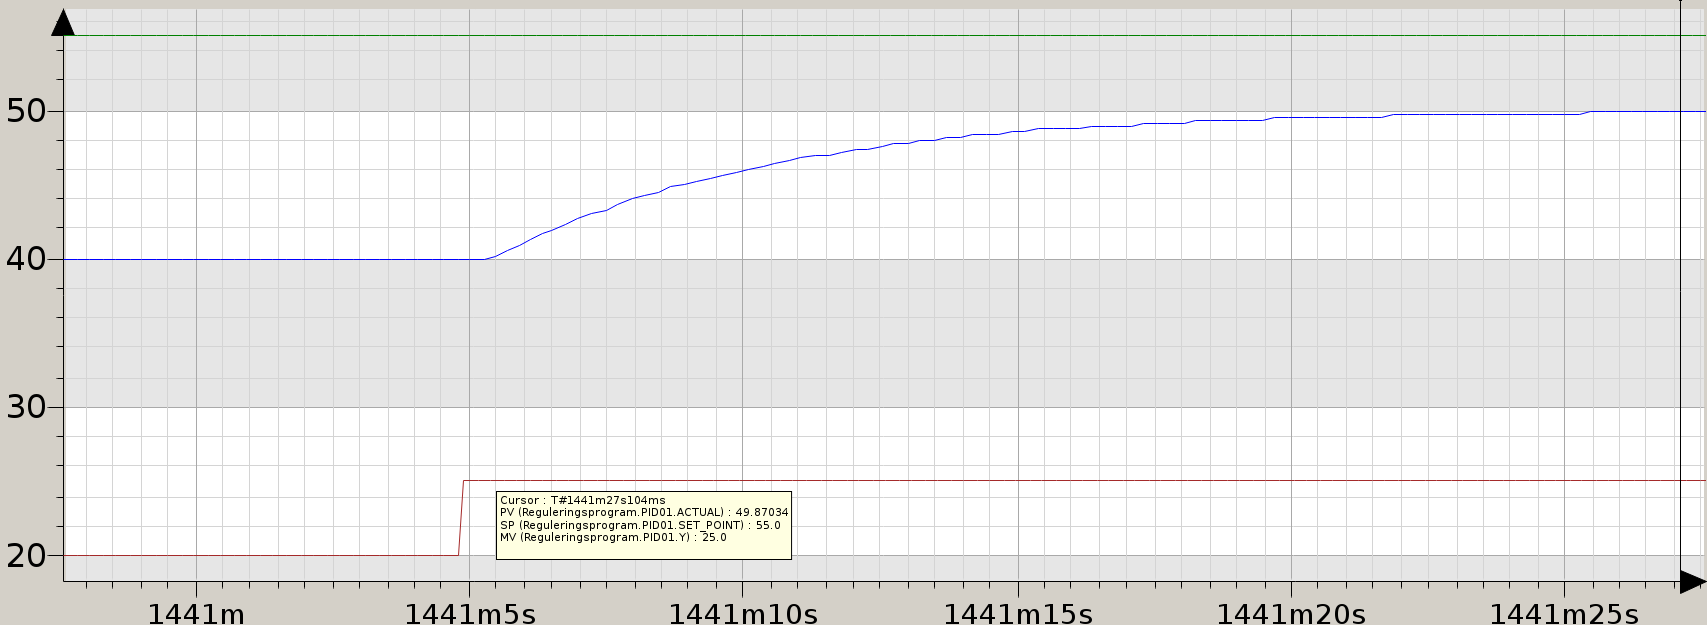
\includegraphics[width=1\textwidth]{Reg_step_response01}

Her er et eksempel på en prosess med tidsforsinkelse. Når vi leser
av garfen får vi at

\begin{eqnarray*}
\theta & = & 0.5s\\
\tau & = & 5s\\
K & = & 2
\end{eqnarray*}

Det gir oss:
\[
K_{P}=\dfrac{\tau}{K\left(T_{C}+\theta\right)}=\dfrac{5}{2(0.5+0.4)}=2.5
\]

c=2 er her mindre en T=5 som gir 
\[
T_{i}=c(T_{c}+\theta)=2(0.5+0.5)=2
\]

Det gir følgende innregulering på et sprang fra 50 til 55. 

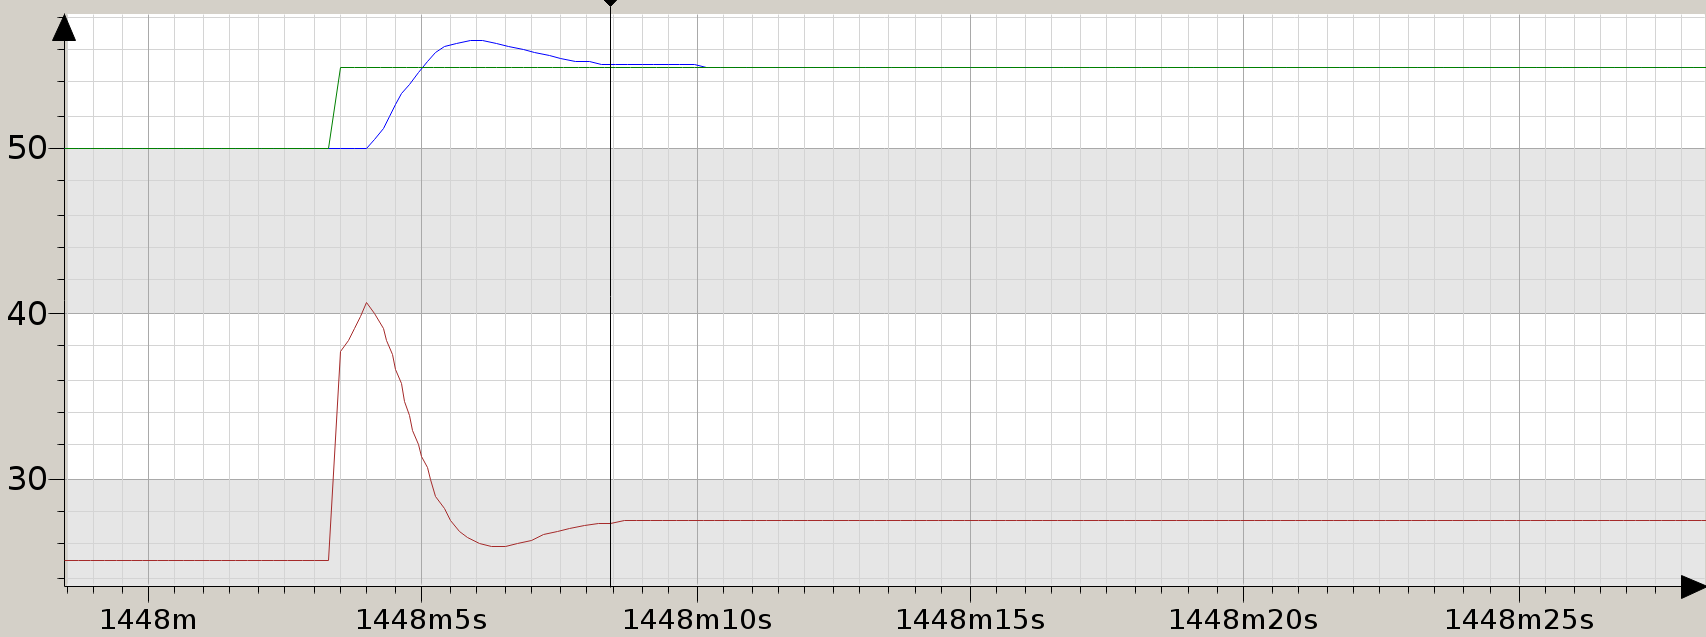
\includegraphics[width=1\textwidth]{Reg_innreg_skogestad01}

\paragraph{Innstilling av PI-regulator for integrator med tidsforsinkelse}

~

\includegraphics{Sprang_integrerendeprosess.eps}

\[
K_{i}=\dfrac{\Delta PV}{\Delta MV\cdot\Delta t}
\]

\[
Kp=\dfrac{1}{K_{i}\left(T_{c}+\theta\right)}
\]

\[
T_{i}=c\left(T_{c}+\theta\right)
\]

Eksempel:

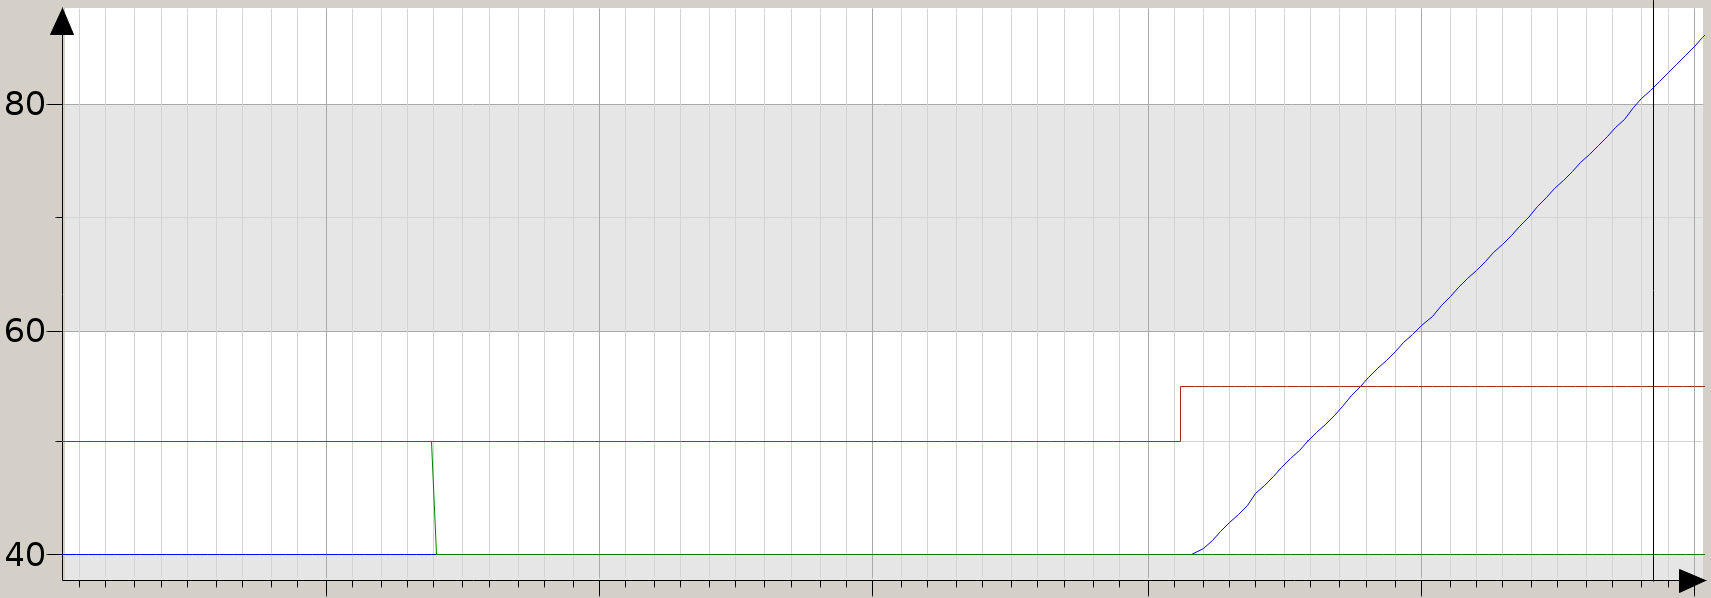
\includegraphics[width=1\textwidth]{Reg_step_integrator}

\[
K_{i}=\dfrac{\Delta PV}{\Delta MV\cdot\Delta t}=\dfrac{40\%}{5\%\cdot8s}=1/s
\]
\[
\tau=0.5s
\]

\[
Kp=\dfrac{1}{K_{i}\left(T_{c}+\theta\right)}=\dfrac{1}{1}
\]

\[
T_{i}=c\left(T_{c}+\theta\right)=2\left(0.5+0.5\right)=2
\]
Som gir følgende innregulering

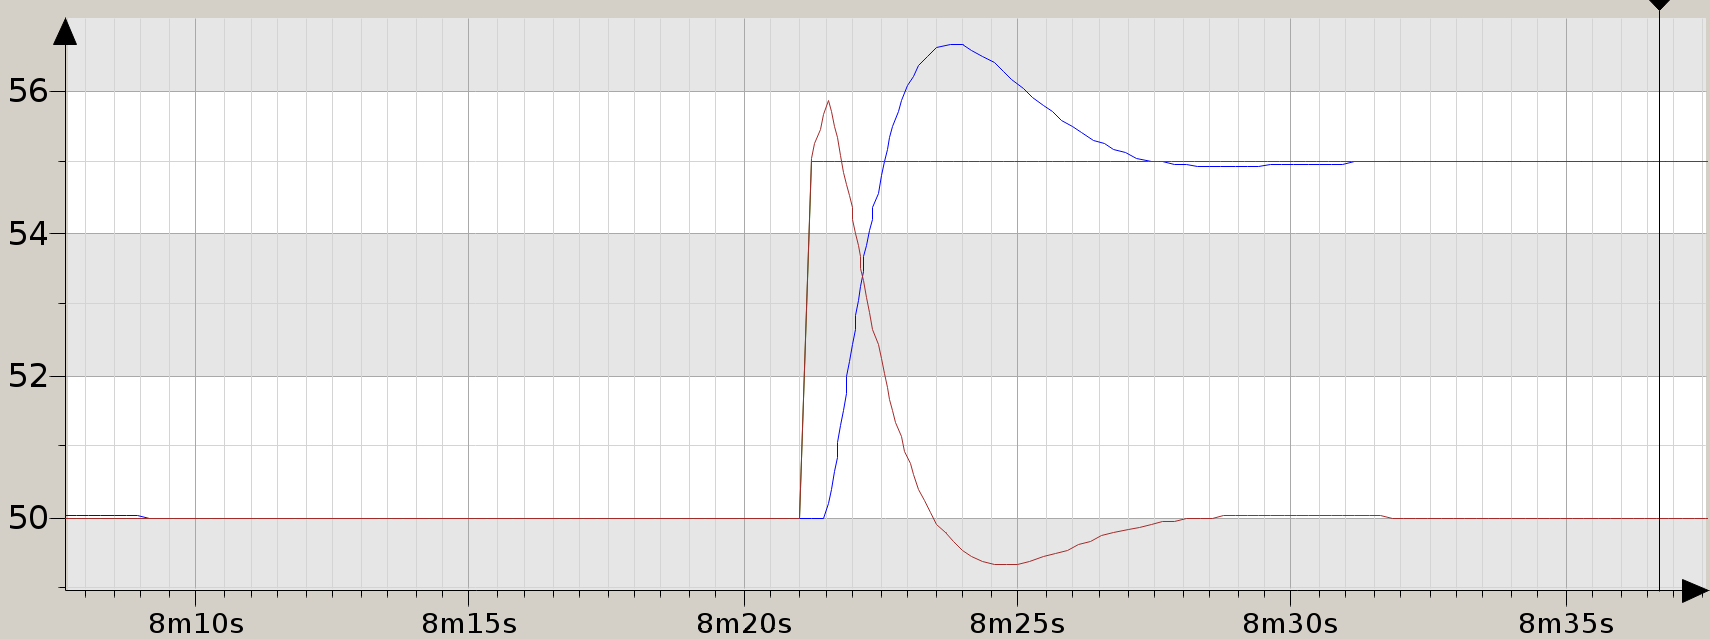
\includegraphics[width=1\textwidth]{Reg_innreg_skogestad02}
\vfil  \eject


\section{Industriroboter}
Hva er en industi robot?

\vskip 5pt 
Industrial robot as defined by iso 8373:2012:
An automatically controlled, reprogrammable, multipurpose manipulator.
Programmable in three or more axes, which can be either fixed in place or mobile for use in industrial automation applications.

\vskip 5pt 
Klassifiskajson av industriroboter ut fra mekanisk struktur. 
\begin{itemize}[noitemsep]
	\item Linære roboter (Cartesian og Gantry)
	\item SCARA robots
	\item Artikulert robot (den vi har)
	\item Parallelle roboter (delta)
\end{itemize}


Classification by mechanical structure:
Linear robots (including cartesian and gantry robots)
SCARA robots
Articulated robots
Parallel robots (delta)
Cylindrical robots
Others
Not classified
Figures 1.1 illustrates the mechanical c

\vskip 10pt 
Hva kjennetegner en industriell robot:
\begin{itemize}[noitemsep]
\item den kjører automatisk
\item den kan reprogrammeres
\item den har en arm med mer en tre akser som en kan feste ulike verktøy på
\item den kan enten stå fast eller være flyttbare
\item den er laget for å løse industrelle oppgaver 
\end{itemize}

Ulike industrielle roboter kan være:
\begin{itemize}[noitemsep]
\item Linære roboter
\item SCARA roboter
\item Parallelle roboter
\item Artikulerte roboter
\item Sylindriske roboter
\item 
\end{itemize}

\vskip 10pt 
Eksempler på industrielle bruksområder:


\begin{itemize}[noitemsep]
\item Forflytting av metall i deleproduksjon eller støyping
\item palletering
\item sveising
\item lakkering
\item pakking
\item automatisk lagersystem
\end{itemize}
\vfil  \eject
\subsection{Robotstudio}

Installasjon:
\begin{itemize}[noitemsep]
	\item Last ned installasjonsfeil fra fagbibliotek
	\item Installer robotware i fra
	\item Koble opp til lisensserver og hent ut en commuter lisens for 90 dager(max).
\end{itemize}


\section{Utstyr}
\subsection{Gand RIO-trainer}

Kortet kobles til PLS med en USB kabel og en trenger en USB til seriel
driver (CH340). 

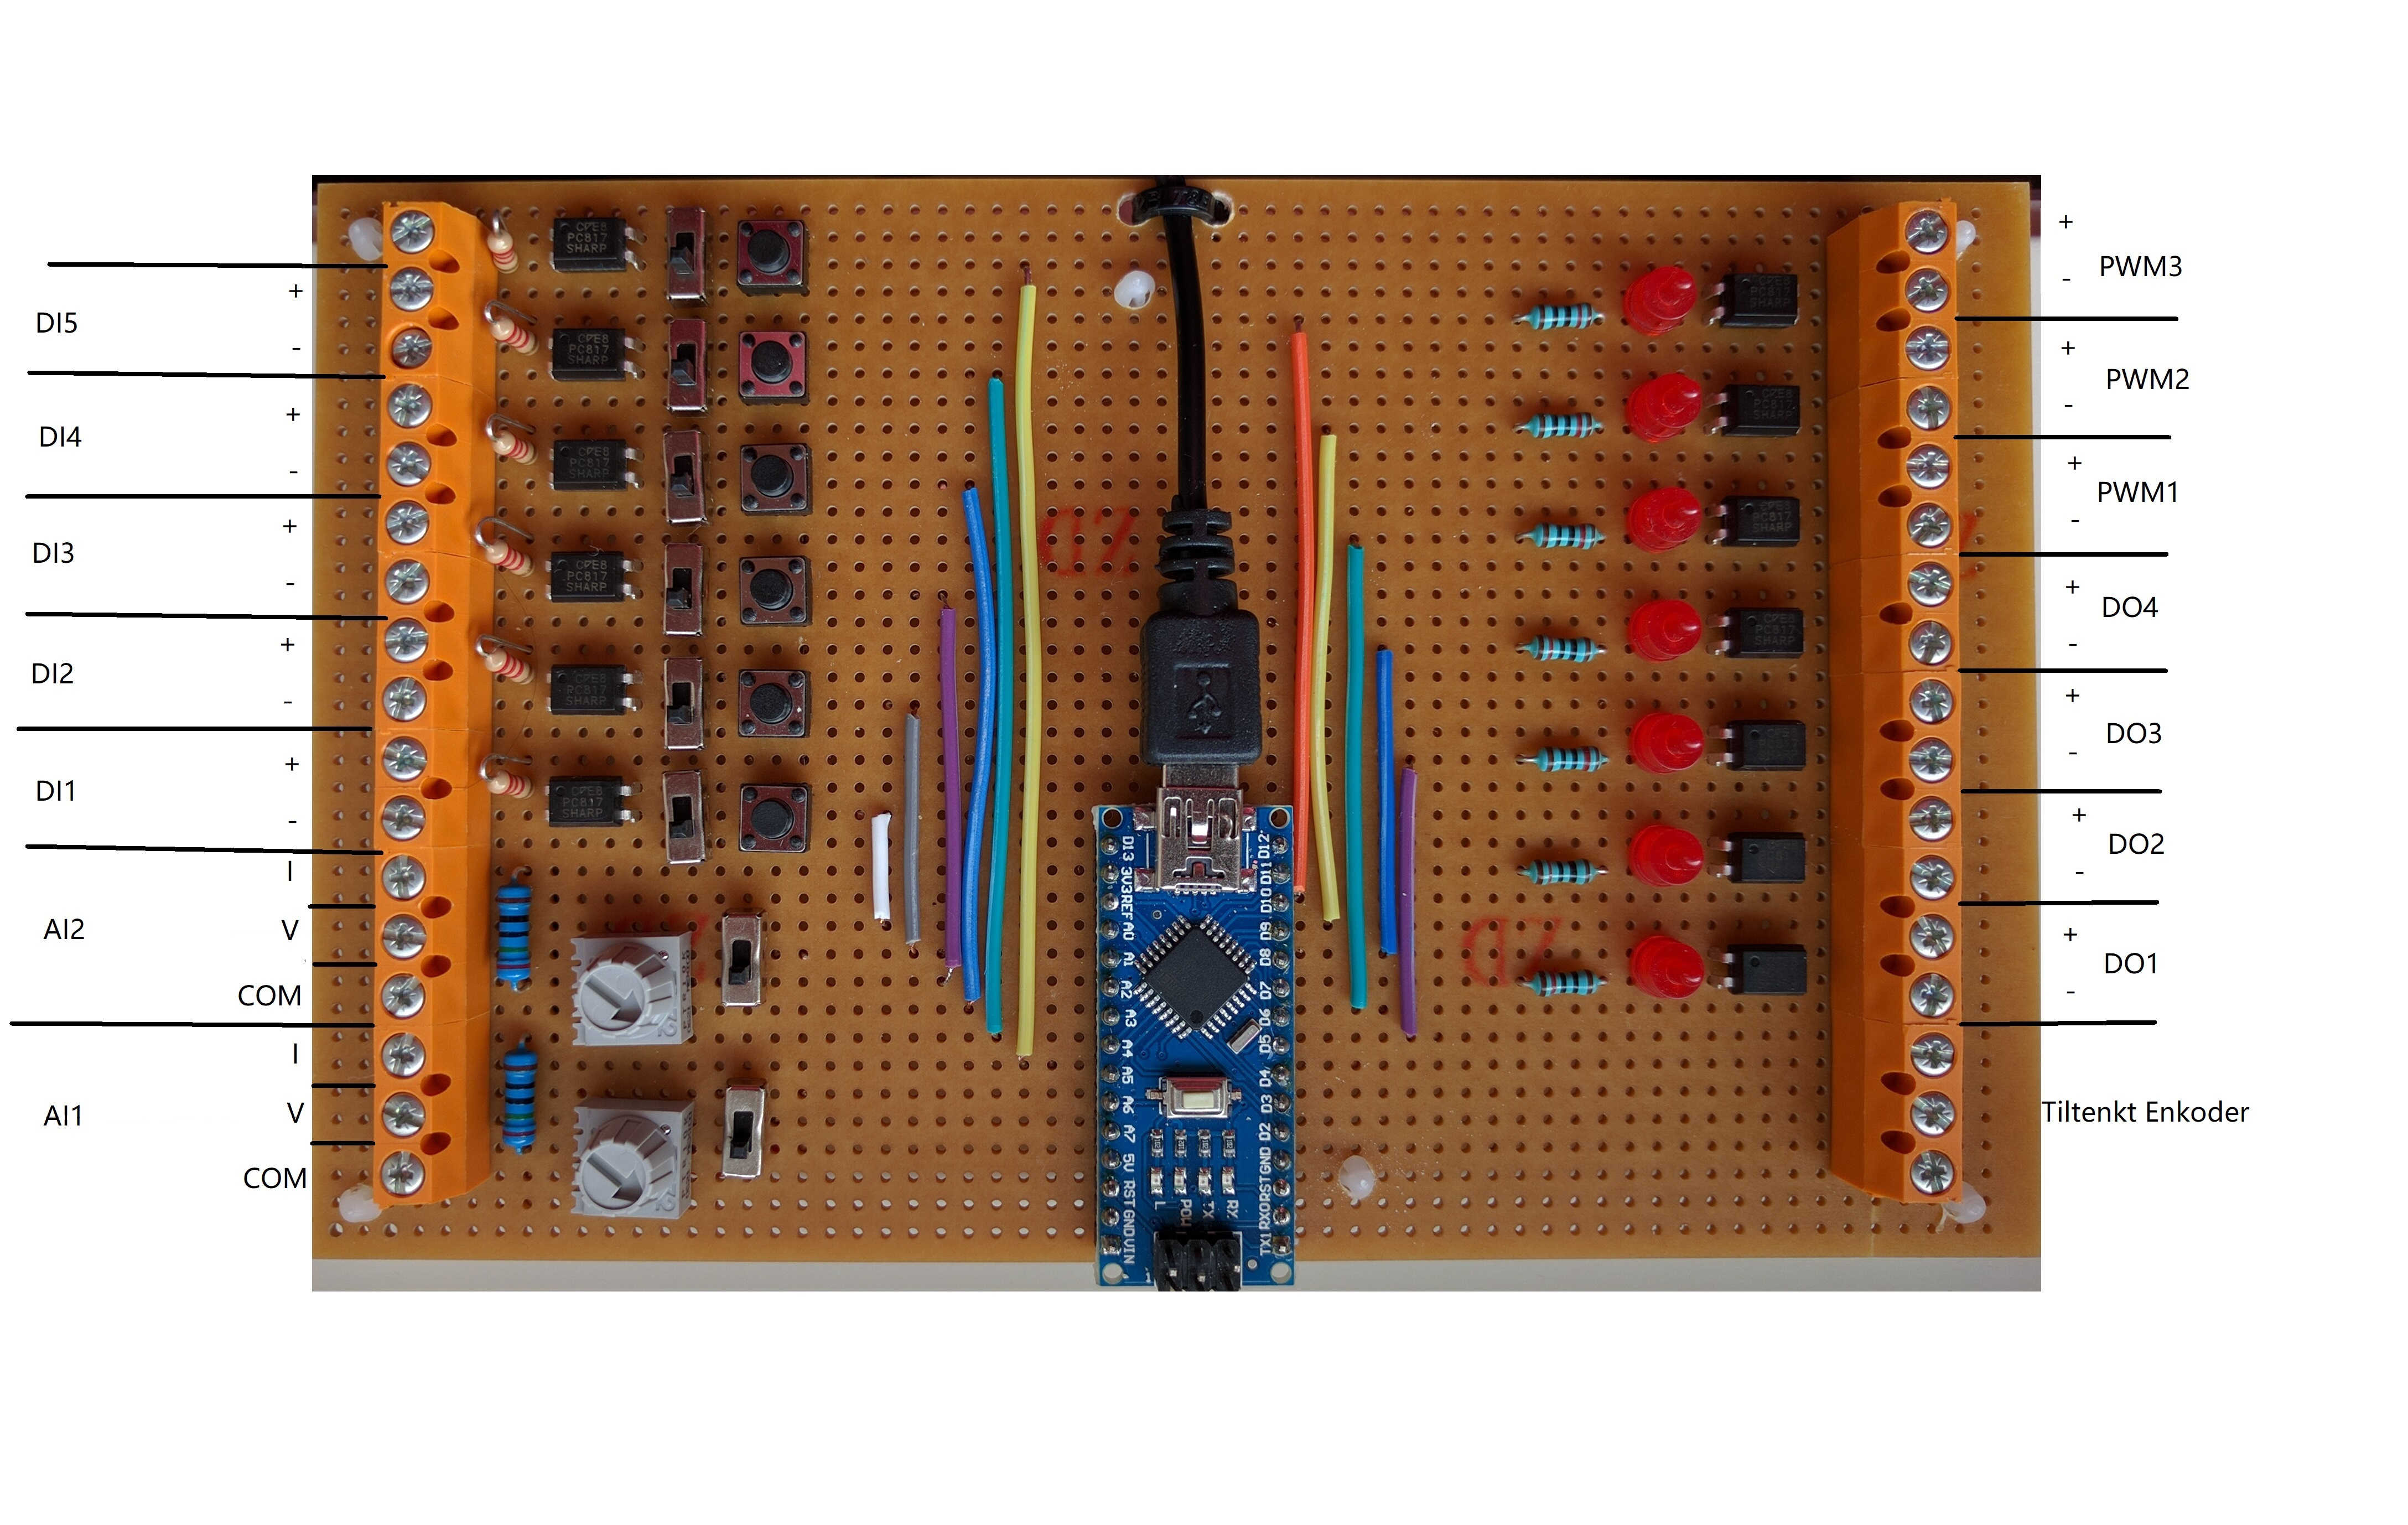
\includegraphics[width=1\textwidth]{./GandRioTrainer.jpg}
\small
\begin{tabular}{|c|c|c|c|}
\hline 
\multicolumn{4}{|c|}{Modbus Data Table}\tabularnewline
\hline 
\hline 
IO & Tilkobling & Register & \tabularnewline
\hline 
Encoder &  & 0000H & Enkoder telleverdi\tabularnewline
\hline 
DO1 & åpen kollektor & 0001H & bit0\tabularnewline
\hline 
DO2 & åpen kollektor & 0001H & bit1\tabularnewline
\hline 
DO3 & åpen kollektor & 0001H & bit2\tabularnewline
\hline 
DO4 & åpen kollektor & 0001H & bit3\tabularnewline
\hline 
PWM1 & åpen kollektor & 0002H & AO 0 (PWM)\tabularnewline
\hline 
PWM2 & åpen kollektor & 0003H & AO 1 (PWM)\tabularnewline
\hline 
PWM3 & åpen kollektor & 0004H & AO 2 (PWM)\tabularnewline
\hline 
DI1 & 24VDC & 0005H & bit0\tabularnewline
\hline 
DI2 & 24VDC & 0005H & bit1\tabularnewline
\hline 
DI3 & 24VDC & 0005H & bit2\tabularnewline
\hline 
DI4 & 24VDC & 0005H & bit3\tabularnewline
\hline 
DI5 & 24VDC & 0005H & bit4\tabularnewline
\hline 
DI6 & 24VDC & 0005H & bit5\tabularnewline
\hline 
AI2 & 4-24mA/0-5V & 0006H & AI2\tabularnewline
\hline 
AI1 & 4-24mA/0-5V & 0007H & AI1\tabularnewline
\hline 
\end{tabular}
\normalsize
\vfil \eject
\subsection{Wago PFC200 på stasjon 3}

Stasjon 3 \\
IP 192.168.0.3\\
web grensesnitt innlogging:\\
user:admin\\
pass:wago\\
\\\\
Codesys innlogging:\\
user:Elev3AUA\\
pass:3AUAGand\\
\section{Instrumenter}
\subsection{multimeter}
\subsection{loop claibrator}
\subsection{nettverkstester}
\subsection{megger}
\subsection{kontinuitetstester}







\section{Formelsamling}

\subsection{Elektroteknikk}
\vskip 2.5pt
\subsubsection*{Ohms lov}
\vskip 2.5pt
$U=R\cdot I$.
\vskip 2.5pt
\subsubsection*{Kirchoffs lover}
\vskip 2.5pt  
Strøm $\Sigma I=0$\\
\vskip 2.5pt  
$I=I_{1}+I_{2}+\cdot\cdot\cdot+I_{n}$\\
\vskip 2.5pt  
$R=\dfrac{1}{\dfrac{1}{R_{1}}+\dfrac{1}{R_{2}}+\cdot\cdot\cdot+\dfrac{1}{R_{n}}}$
\vskip 2pt
 Spenning $\Sigma U=0$\\
\vskip 2.5pt  
$U=U_{1}+U_{2}+\cdot\cdot\cdot+U_{n}$\\
\vskip 2.5pt  
$R=R_{1}+R_{2}+\cdot\cdot\cdot+R_{n}$\\
\vskip 2pt
Lederresistans: $ R=\frac{\rho\cdot l}{A}$ 
\vskip 2pt
Kortsluttningstrøm $I_{k}=\frac{E}{R_{i}+R_{ytre}}$
\vskip 2pt
Elektrisk effekt: $P=\frac{W}{t}$
\vskip 2pt  
Effektloven: $P=U\cdot I\cdot \sqrt{3} \cdot \cos \varphi$
\vskip 2.5pt  
Virkningsgrad: $\eta=\frac{P_{avgitt}}{P_{tilf\\ort}}$
\vskip 2.5pt
Synkron hastihet: $n_1=\frac{2\cdot f}{P}$
\vskip 2.5pt 
Sakking: $S=\frac{n_1-n}{n_1}$
\vskip 2.5pt 
\subsection{Reguleringsteknikk}
\vskip 2.5pt 
\subsubsection*{PID-regulator}
$MV=$\\
$K_p(e+1/TN \int e dt + TV de/dt)+BIAS$\\
\vskip 2.5pt
$Direkte e=PV-SP$\\
$Reverserende e=SP-PV$\\
\subsubsection*{Ziegler \& Nichols svingemetode}
\subsubsection*{P-regulator}
$K_p = 0.5\cdot K_u$
\subsubsection*{PI-regulator}
$K_p = 0.45\cdot K_u$\\
$T_i = 0,83\cdot T_u$\\
\subsubsection*{PID-regulator}
$K_p = 0.6\cdot K_u$\\
$T_i = 0,5\cdot T_u$\\
$T_d = 0,125\cdot T_u$\\
\vskip 2.5pt 
\subsubsection*{Prosessdynamikk}
\vskip 2.5pt 
$\theta$=døtid
\vskip 2.5pt 
$ \text{Tidskonstant finnes når} \Delta PV_{63\%}$
\vskip 2.5pt 
$\tau$=tidskonstand
\vskip 2.5pt 
$T_C$ velges lik $\theta$
\vskip 2.5pt 
\subsubsection*{Selvstabiliserende}
\vskip 2.5pt 
$K=\dfrac{\Delta PV}{\Delta MV} $
\vskip 2.5pt 
$K_p=\dfrac{\tau}{K(T_C+\theta)}$
\vskip 2.5pt 
$T_i=2(T_C+\theta)$
\vskip 2.5pt 
\subsubsection*{Integrerende}
\vskip 2.5pt 
$K_i=\dfrac{\Delta PV}{\Delta MV \cdot {\Delta t}}$
\vskip 2.5pt 
$K_p=\dfrac{1}{K_i(T_C+\theta)}$
\vskip 2.5pt 
$T_i=2(T_C+\theta)$\\
\subsection{Måleteknikk}
\subsubsection*{Kalibrering}
Feilprosent av span:\\
$Error=\frac {IUT-Standard}{Span} \cdot 100\% $\\
\vskip 2.5pt 
Skaleringsformel:
\vskip 2.5pt 
$\dfrac{x-x_{start}}{x_{range}}=\dfrac{y-y_{start}}{y_{range}}$\\
Eksempel: $\dfrac{12mA-4mA}{16mA}=\dfrac{50\%-0\%}{100\%}$
\subsubsection*{Flowmåling}
\vskip 2.5pt 
\vskip 2.5pt 
\vskip 2.5pt 
Reynoldstall: $Re=\dfrac {D \cdot v \cdot \rho}{\mu}$\\
\vskip 2.5pt 
Bernoulli's formel:\\
$z_1 \rho g + {v_1^2 \rho \over 2} + P_1 = z_2 \rho g + {v_2^2 \rho \over 2} + P_2$\\
\vskip 2.5pt 
\subsubsection*{Law of Continuity}
$\rho_1 A_1 \overline{v_1} = \rho_2 A_2 \overline{v_2} = \cdots \rho_n A_n \overline{v_n}$\\
\\
$W = \rho A \overline{v}$\\\\
$Q=A_1 \overline{v_1} = A_2 \overline{v_2}$\\

Massestrøm: $W=\frac{m}{t}$\\
\vskip 2.5pt 
Volumstrøm: $Q=\frac{V}{t}$\\
\vskip 2.5pt 
Massetetthet: $\rho=\frac{m}{V}$\\
\vskip 2.5pt 
\subsubsection*{Trykkbaserte strømningsmålere}
Måleblende: $Q=k\cdot \sqrt{\Delta p}$\\
\vskip 2.5pt 
Måleblende med varierende $\rho$: $Q=k\cdot \sqrt{\frac{\Delta p}{\rho}}$\\
\vskip 2.5pt
Kvadratrot uttrekker:\\
s = signal i prosent (0-1)\\
$s_{ut}=\sqrt{s_{inn}}$\\
\subsubsection*{Hastighetsbaserte strømningsmålere}
Turbin og Vortex:\\
$Q=kf$\\
Elektromagnetisk:\\
$E=Blv$\\
Ultralyd:\\
$Q = k {t_{up} - t_{down} \over (t_{up})(t_{down})}$\\
 
\subsection{Nivåmåling}

$P = \rho \cdot g \cdot h $\\
\subsection{Temperaturmåling}
$R_T = R_{ref}[1 + \alpha(T - T_{ref})]$\\
European $\alpha=0.00385$\\
American $\alpha=0.00392$\\
\vfil \eject


\section{Tabeller}
\includegraphics[width=1\textwidth]{002.eps}
\vfil \eject
\includegraphics[angle=90,height=1\textheight]{./chemistry12.eps}
\vfil \eject
\includegraphics[width=1\textwidth]{calibrate03.eps}
\includegraphics[width=1\textwidth]{calibrate04.eps}
\includegraphics[width=0.5\textwidth]{current09.eps}
\includegraphics[width=0.5\textwidth]{current10.eps}
\includegraphics[width=0.5\textwidth]{current11.eps}
\includegraphics[width=0.5\textwidth]{current12.eps}
\includegraphics[width=0.5\textwidth]{current13.eps}
\includegraphics[width=0.5\textwidth]{current29.eps}
\includegraphics[width=0.5\textwidth]{current30.eps}
\includegraphics[width=0.5\textwidth]{current31.eps}
\includegraphics[width=1\textwidth]{plc_048.eps}
\includegraphics[width=1\textwidth]{plc_052.eps}
\includegraphics[width=1\textwidth]{pressure76.eps}

\vfil \eject
\end {document}
